%!TEX root = ../Report.tex
\subsection{Sample Input \& System Output} % (fold)
\label{sub:appendix_a}

	\subsubsection{Scenario 1} % (fold)
	\label{ssub:scenario_1}
		Parent, Singaporean Male, aged 45, 120,000 annual income.

		Prefers Citibank/Maybank, Visa/MasterCard \& Cashback, Spends 600, 400 \& 200 on Dining, Groceries \& Petrol respectively.

		\textit{Shown below, as user chooses only Maybank as the preferred bank}

		\begin{figure}[H]
			\centering
			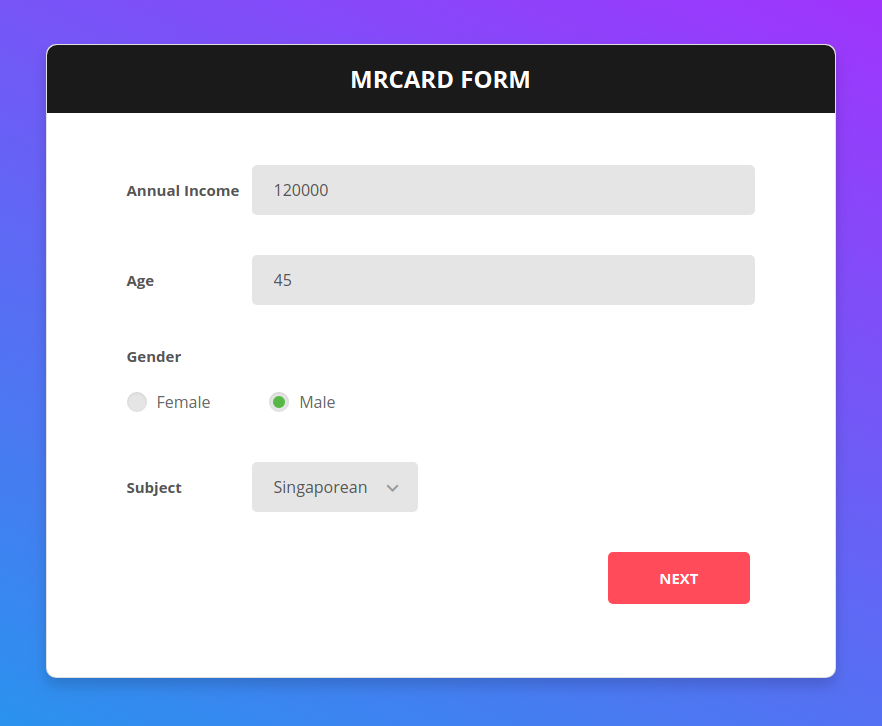
\includegraphics[width=\linewidth]{img/scenario1_eligibility.png}
		\end{figure}

		\begin{figure}[H]
			\centering
			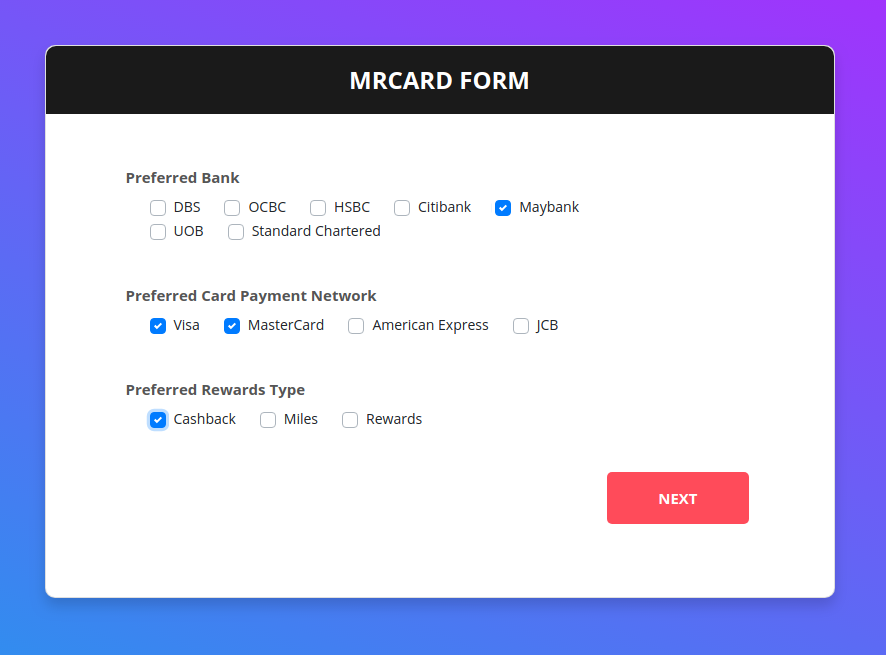
\includegraphics[width=\linewidth]{img/scenario1_preferences_v2.png}
		\end{figure}

		\begin{figure}[H]
			\centering
			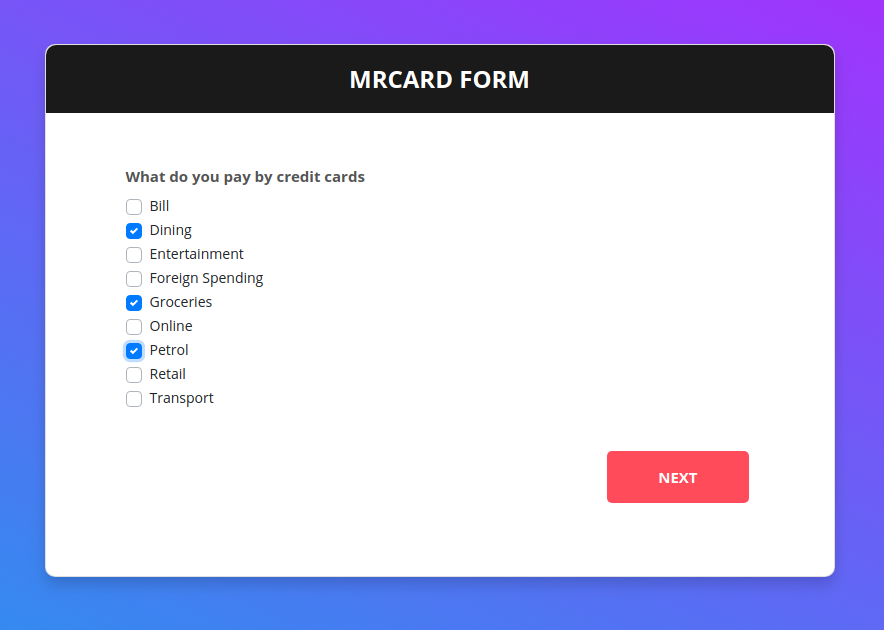
\includegraphics[width=\linewidth]{img/scenario1_spending_checkbox.png}
		\end{figure}

		\begin{figure}[H]
			\centering
			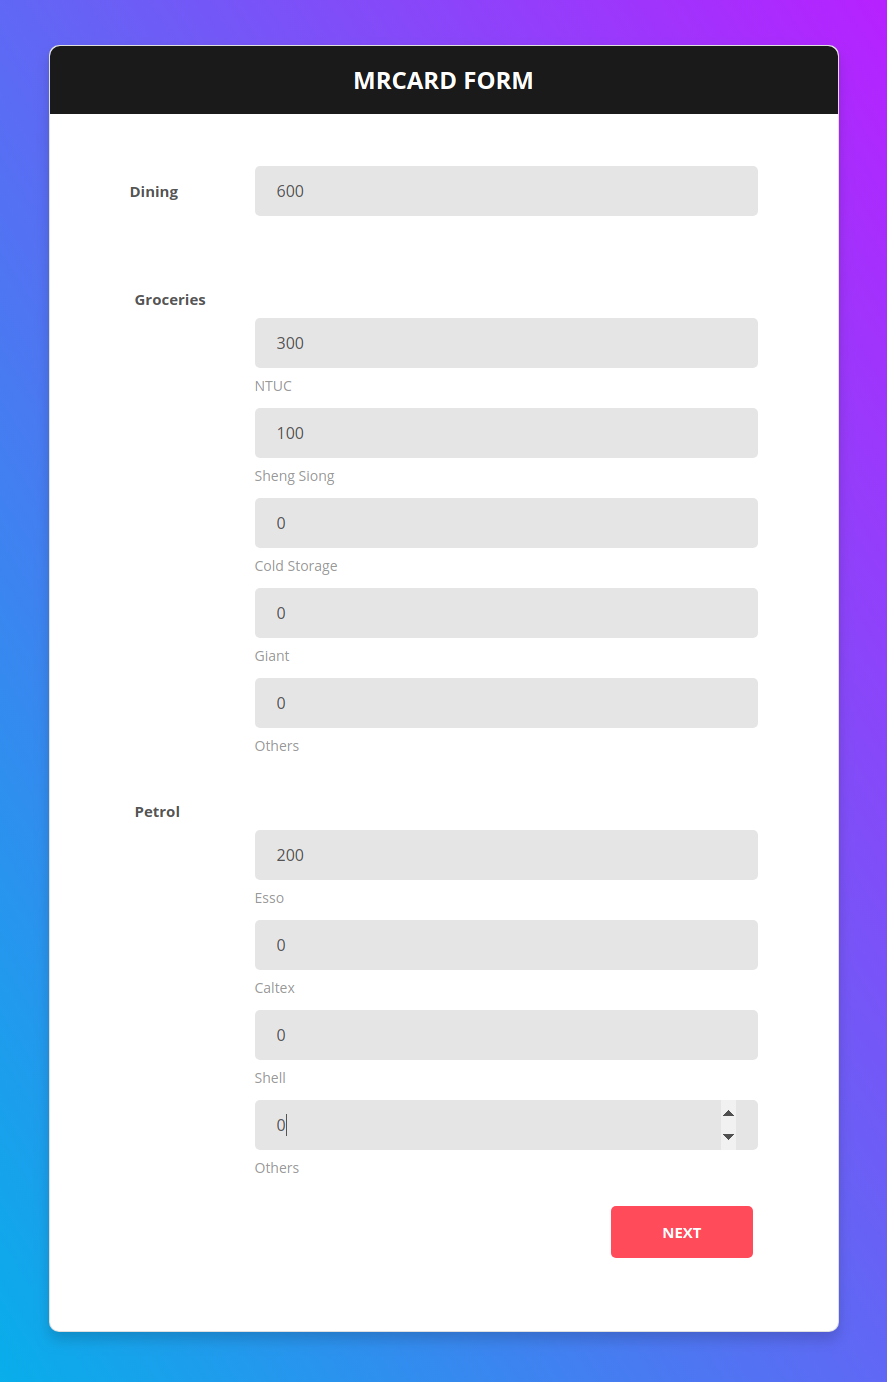
\includegraphics[width=\linewidth]{img/scenario1_spending_amount.png}
		\end{figure}

		\begin{figure}[H]
			\centering
			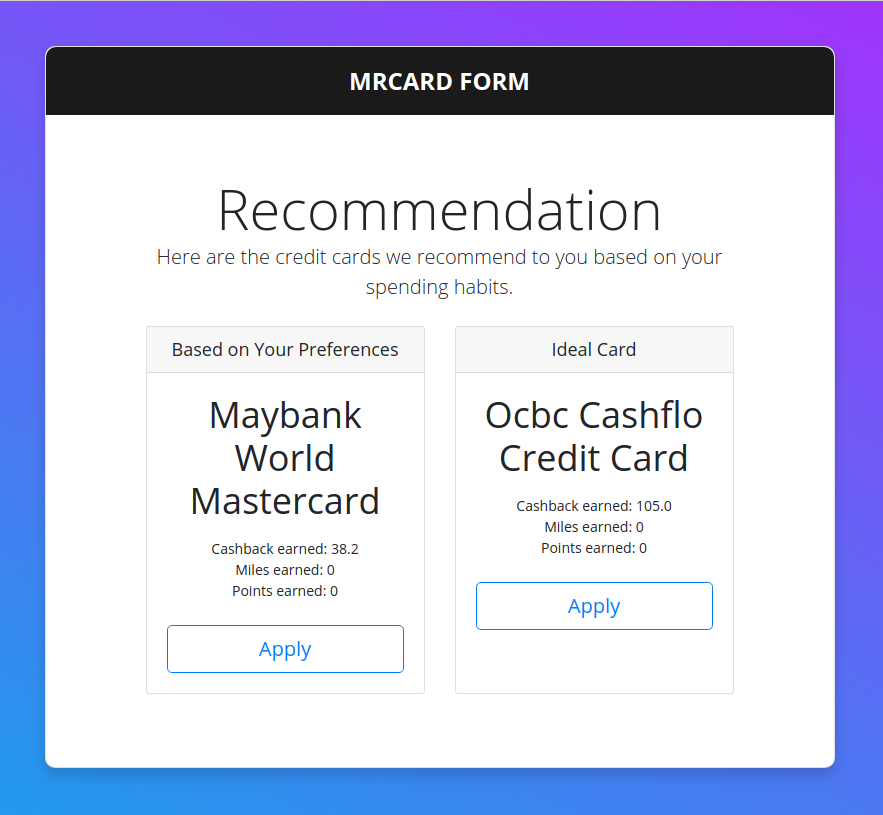
\includegraphics[width=\linewidth]{img/scenario1_recommendation_v2.png}
		\end{figure}

		\begin{figure}[H]
			\centering
			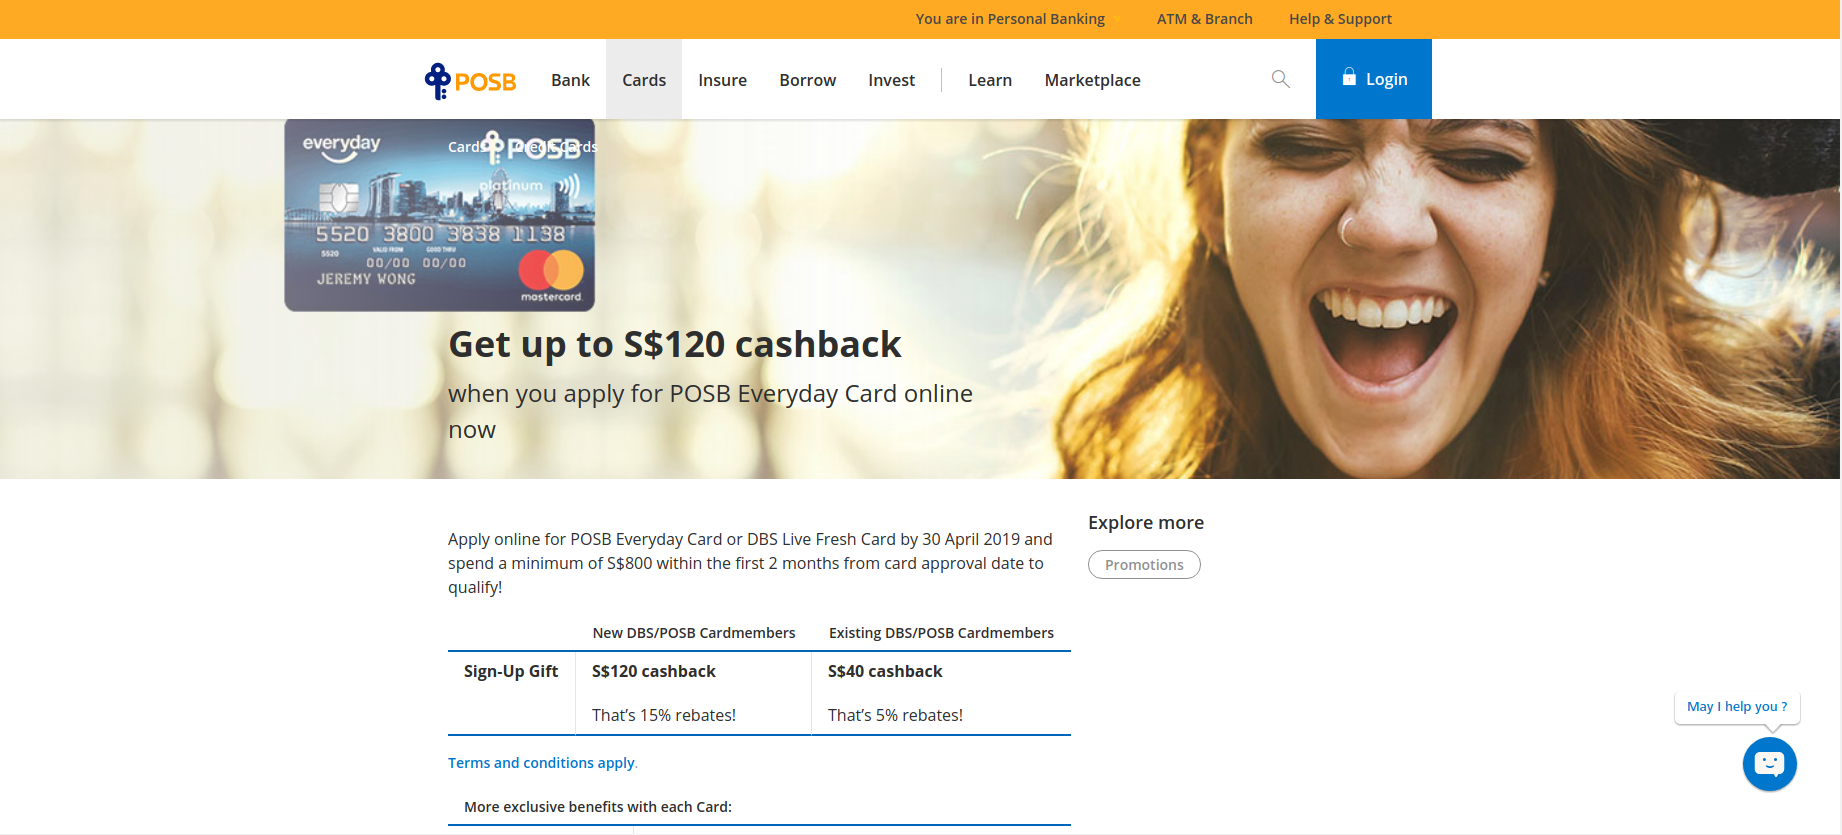
\includegraphics[width=\linewidth]{img/scenario1_apply_ideal_credit_card.png}
		\end{figure}

	% subsubsection scenario_1 (end)

	\subsubsection{Scenario 2} % (fold)
	\label{ssub:scenario_2}
		DBS Staff, Foreigner Female, aged 31, 80,000 annual income.

		Prefers DBS, uses Recommender System to target individuals who like Entertainment and Online Shopping.

		\begin{figure}[H]
			\centering
			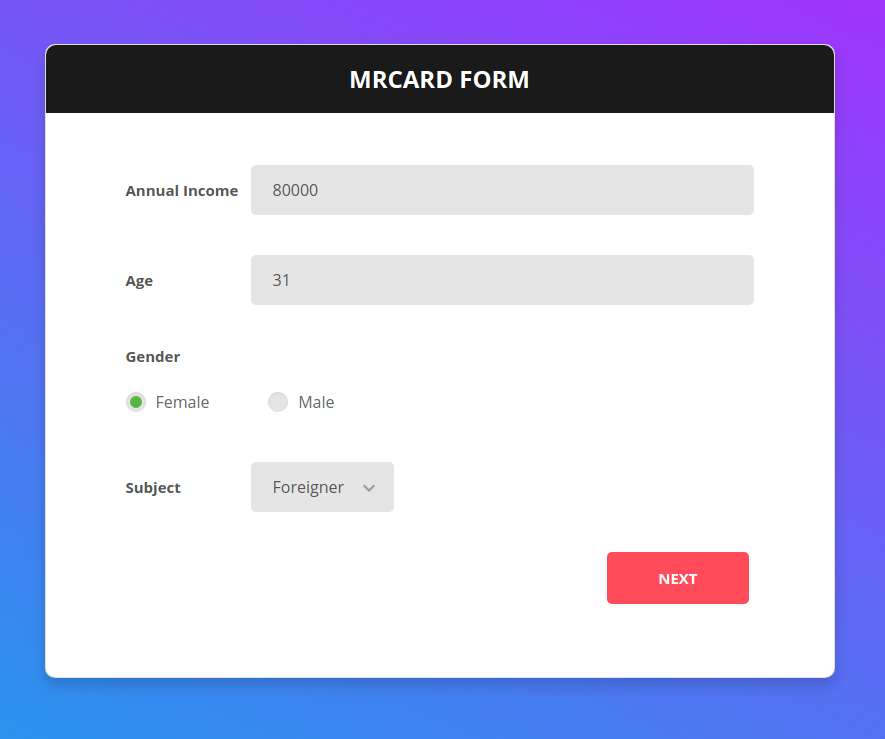
\includegraphics[width=\linewidth]{img/scenario2_eligibility.png}
		\end{figure}

		\begin{figure}[H]
			\centering
			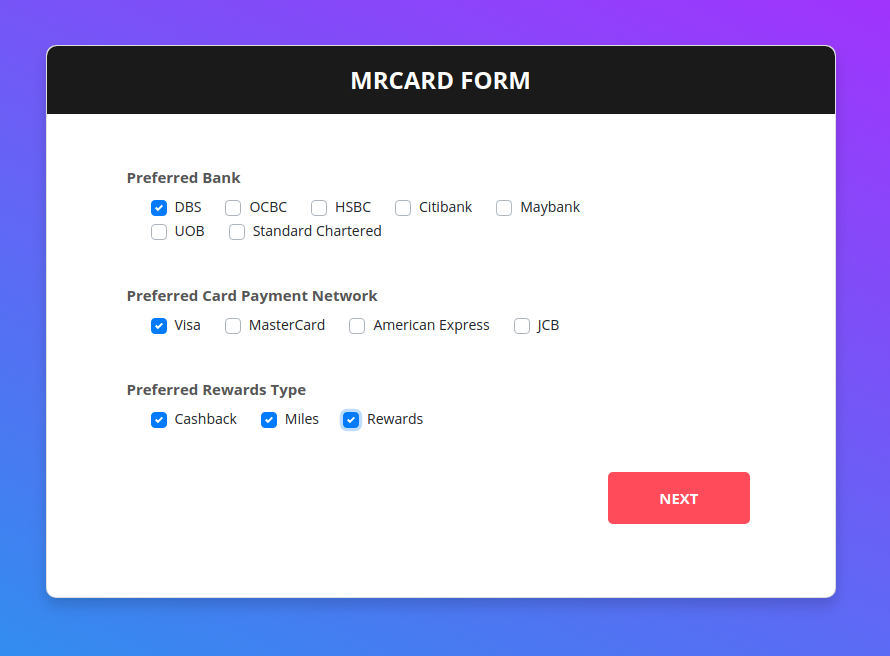
\includegraphics[width=\linewidth]{img/scenario2_preferences.png}
		\end{figure}

		\begin{figure}[H]
			\centering
			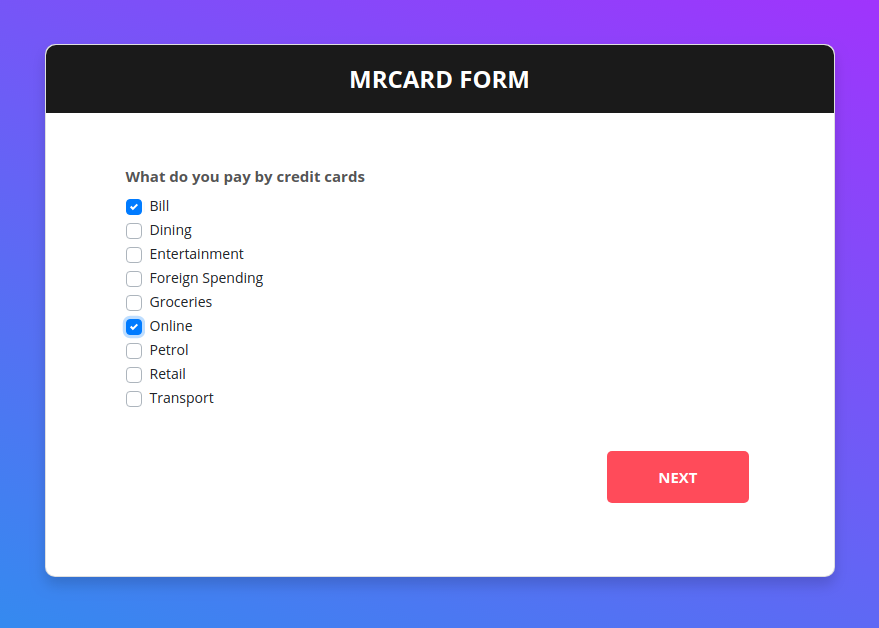
\includegraphics[width=\linewidth]{img/scenario2_spending_checkbox.png}
		\end{figure}

		\begin{figure}[H]
			\centering
			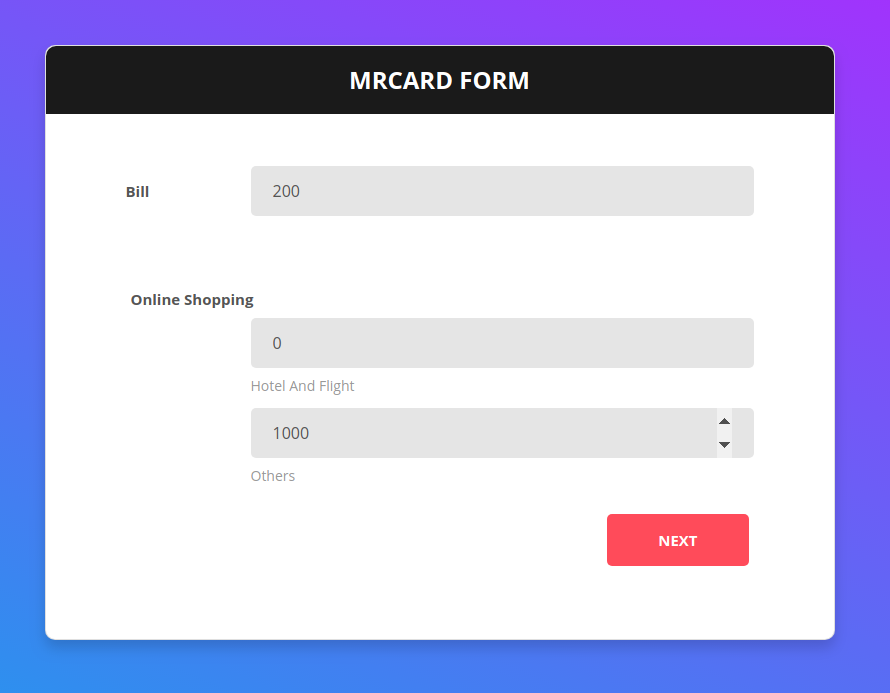
\includegraphics[width=\linewidth]{img/scenario2_spending_amount.png}
		\end{figure}

		\begin{figure}[H]
			\centering
			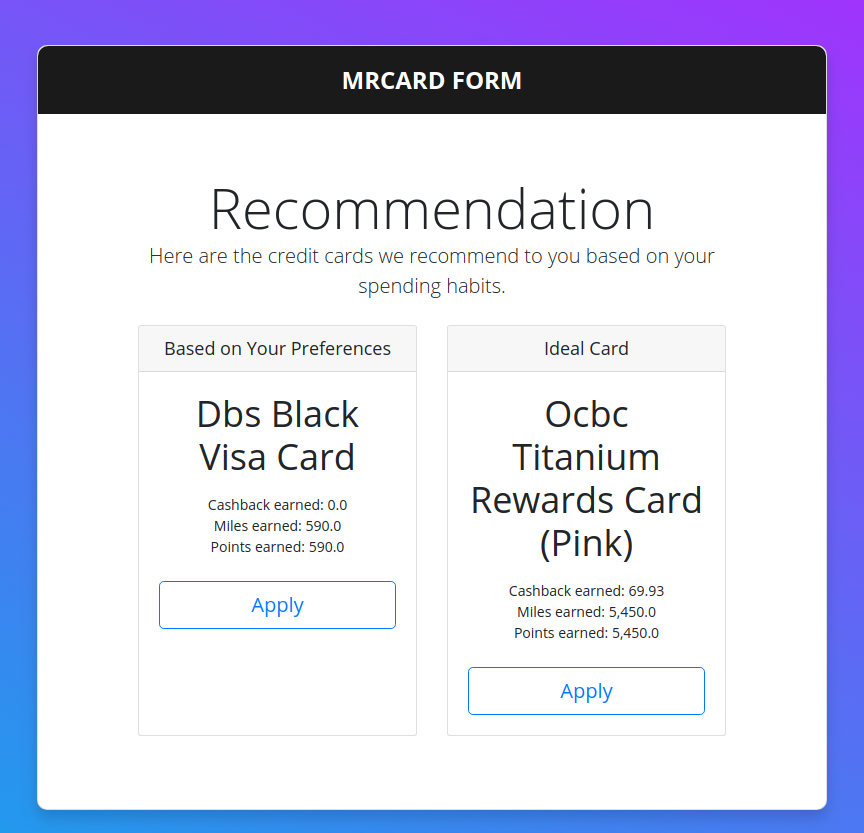
\includegraphics[width=\linewidth]{img/scenario2_recommendation.png}
		\end{figure}
	% subsubsection scenario_2 (end)

	\subsubsection{Scenario 3} % (fold)
	\label{ssub:scenario_3}
		Student, PR Female, aged 19, no annual income. Not eligible for any Credit Cards.

		\textit{Show below, as user is under the minimum age of 21 and/or does not meet the minimum annual income of 20000 SGD, she is not eligibile for any Credit Card.}

		\begin{figure}[H]
			\centering
			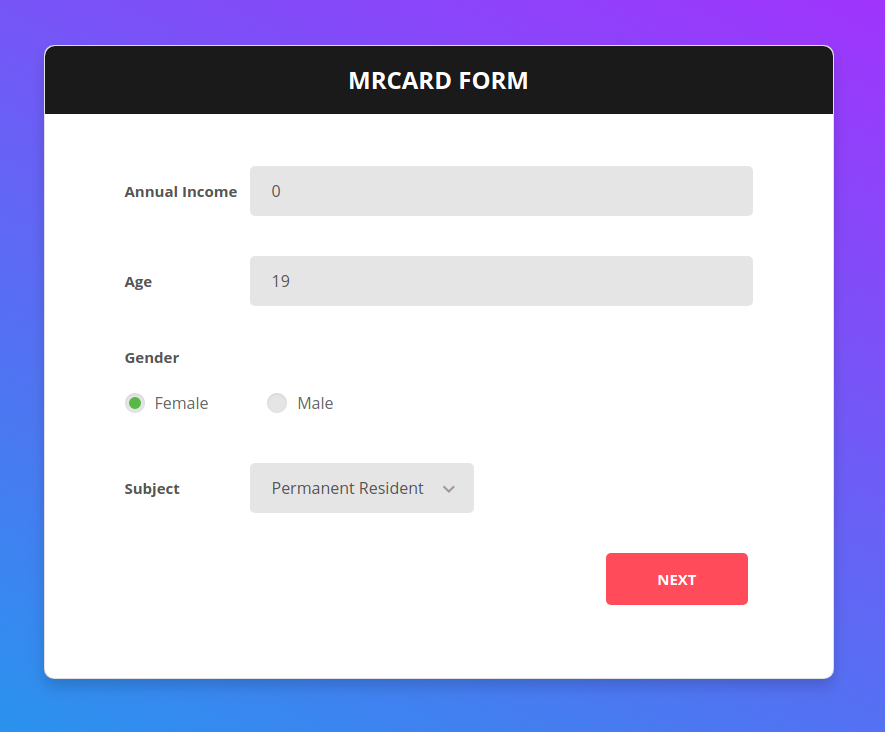
\includegraphics[width=\linewidth]{img/scenario3_eligibility.png}
		\end{figure}

		\begin{figure}[H]
			\centering
			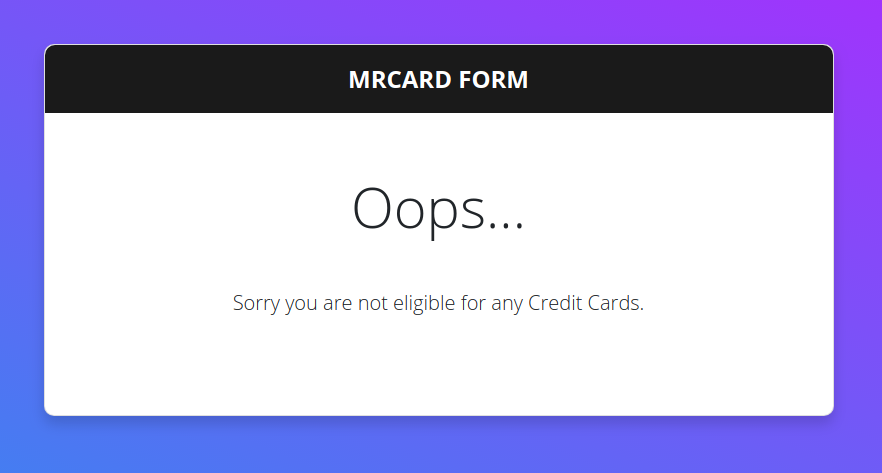
\includegraphics[width=\linewidth]{img/scenario3_no_recommendation.png}
		\end{figure}
	% subsubsection scenario_3 (end)
% subsection appendix_a (end)

% User Manual
\subsection{User's Manual} % (fold)
\label{sub:appendix_b}

	% System Overview
	\subsubsection{System Overview}
	MRCard is a web based \textbf{Credit Card Recommender System}. The target users would be divided into two groups, consumers and businesses. To consumers, it would be a good system to learn what credit card is most suitable base on their spending habits and preferences. To businesses, i.e.\ banks, it would be a professional system to learn how their credit cards are compared with the market competitors. The system would be run with a web UI and it is device-friendly. The users could connect it through Internet and answer some survey question to get the recommendation on credit cards.

	% Supports
	\subsubsection{Supported browsers}

		% Mobile Devices
		\subsubsubsection{Mobile devices}
		It supports the latest versions of each major platform’s default browsers. Note that proxy browsers (such as Opera Mini, Opera Mobile’s Turbo mode, UC Browser Mini, Amazon Silk) are not supported.

			\begin{table}[h]
			\captionsetup{font=scriptsize}
			\centering
			\resizebox{\textwidth}{!}{%
			\begin{tabular}{llllp{4cm}l}
			\toprule
			                           & \textbf{Chrome} & \textbf{Firefox} & \textbf{Safari} & \textbf{Android Browser \& WebView} & \textbf{Microsoft Edge} \\ \midrule
			\textbf{Android}           & Supported       & Supported        & N/A             & Android v5.0+ supported             & Supported               \\
			\textbf{iOS}               & Supported       & Supported        & Supported       & N/A                                 & Supported               \\
			\textbf{Windows 10 Mobile} & N/A             & N/A              & N/A             & N/A                                 & Supported               \\ \bottomrule
			\end{tabular}%
			}
			\caption{Mobile Devices Support}
			\label{mobile-support}
			\end{table}

		% Desktop Browsers
		\subsubsubsection{Desktop browsers}
		The latest versions of most desktop browsers are supported.

			\begin{table}[h]
			\captionsetup{font=scriptsize}
			\centering
			\resizebox{\textwidth}{!}{%
			\begin{tabular}{@{}lllllll@{}}
			\toprule
			                 & \textbf{Chrome} & \textbf{Firefox} & \textbf{Internet Explorer} & \textbf{Microsoft Edge} & \textbf{Opera} & \textbf{Safari} \\ \midrule
			\textbf{Mac}     & Supported       & Supported        & N/A                        & N/A                     & Supported      & Supported       \\
			\textbf{Windows} & Supported       & Supported        & Supported, IE10+           & Supported               & Supported      & Not supported   \\ \bottomrule
			\end{tabular}%
			}
			\caption{Desktop Browser Support}
			\label{desktop-support}
			\end{table}

	% Deployment system define
	\subsubsection{Deployment}
	Our system is deployed by Django, which is a Python-based free and open-source web framework. To run the system successfully, some basic packages are required with the latest version of Python 3 (i.e.\ Python 3.7.2).

	% TODO packages
	\textbf{Packages:}
	\begin{itemize}
		\item PyKnow
		\item panda
		\item Django
	\end{itemize}

	Once the running environment is ready, please open the system folder in terminal, and run the command \verb|python3 manage.py runserver|. You should see the following output on the command line:

	\begin{lstlisting}[style=DOS, frame=single, gobble=7, tabsize=4, showstringspaces=false]
		Performing system checks...

		System check identified no issues (0 silenced).

		You have unapplied migrations; your app may not work properly
		until they are applied.
		Run 'python manage.py migrate' to apply them.

		February 28, 2019 - 15:50:53
		Django version 2.1, using settings 'mysite.settings'
		Starting development server at http://127.0.0.1:8000/
		Quit the server with CONTROL-C.
	\end{lstlisting}

	Then you can go to the web browser and input URL "http://127.0.0.1:8000/" to use MRCard.

	% TODO Pictures and steps here

	\subsubsection{Procedure} % (fold)
	\label{ssub:start}
		Open up your preferred browser and go to the URL “http://127.0.0.1:8000/” as shown below:

		\begin{figure}[H]
			\centering
			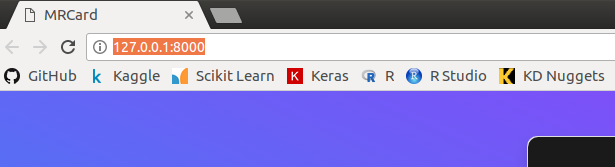
\includegraphics[width=\linewidth]{img/url.png}
		\end{figure}

		Input your Annual Income (rough), Age, Gender and Citizenship, they are all required fields. We use this to calculate which Credit Cards you are eligible for.

		\begin{figure}[H]
			\centering
			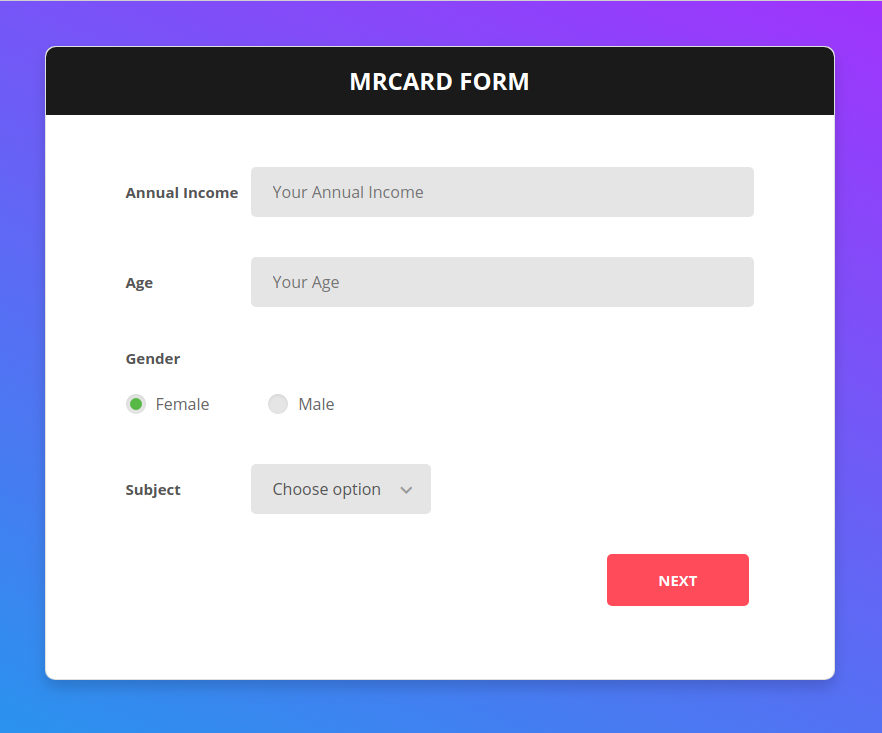
\includegraphics[width=\linewidth]{img/eligibility.png}
		\end{figure}

		Input your Annual Income (rough), Age, Gender and Citizenship are all required fields. If you do not fill in a given field, a prompt will be exposed to remind you.

		\begin{figure}[H]
			\centering
			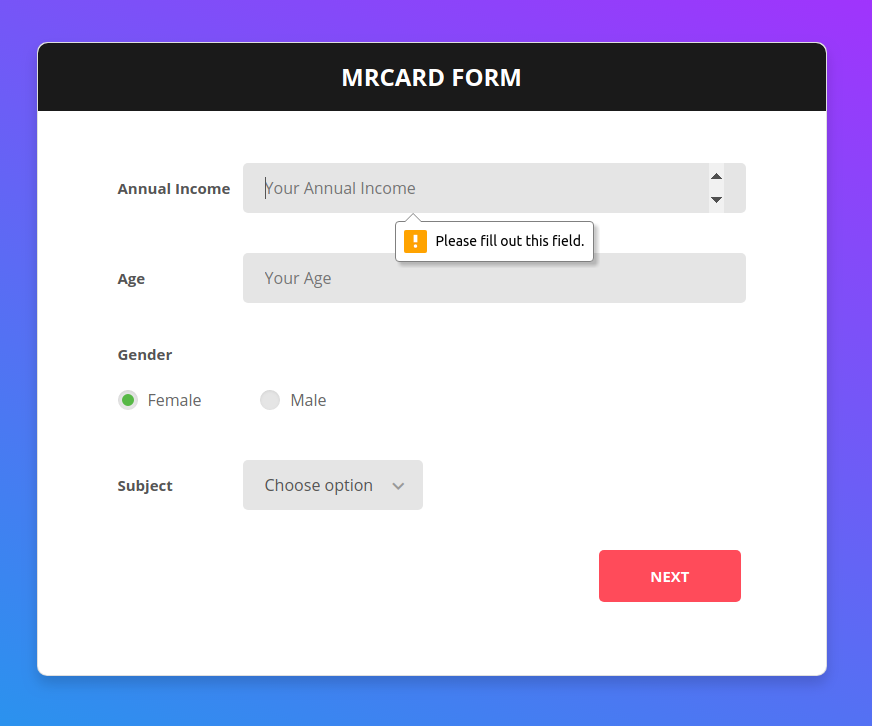
\includegraphics[width=\linewidth]{img/eligibility_fill_in.png}
		\end{figure}

		Next, you get to choose which Bank/ Payment Network and Rewards type you prefer. We will include this as part of the recommendation for preferred cards, together with the ideal Credit Card. From the set of eligible Cards, we recommend an ideal card. And from the set of eligible and preferred Credit Cards, we recommend a preferred card.

		\begin{figure}[H]
			\centering
			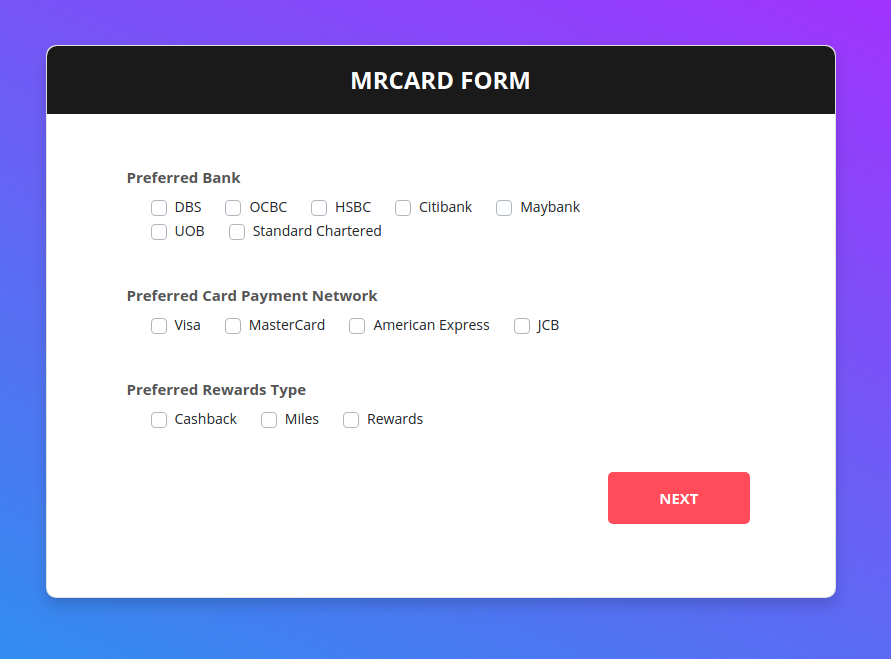
\includegraphics[width=\linewidth]{img/preferences.png}
		\end{figure}

		Following which, click on which categories you spend on with a Credit Card. We use this internally so that we don’t need to ask you unnecessary questions for categories that you don’t spend on. (e.g. If you select Groceries, we will ask you how much you spend on it) We also have a more granular breakdown for certain categories because the breakdown matters when calculating Cashback/ Miles/ Rewards.

		\begin{figure}[H]
			\centering
			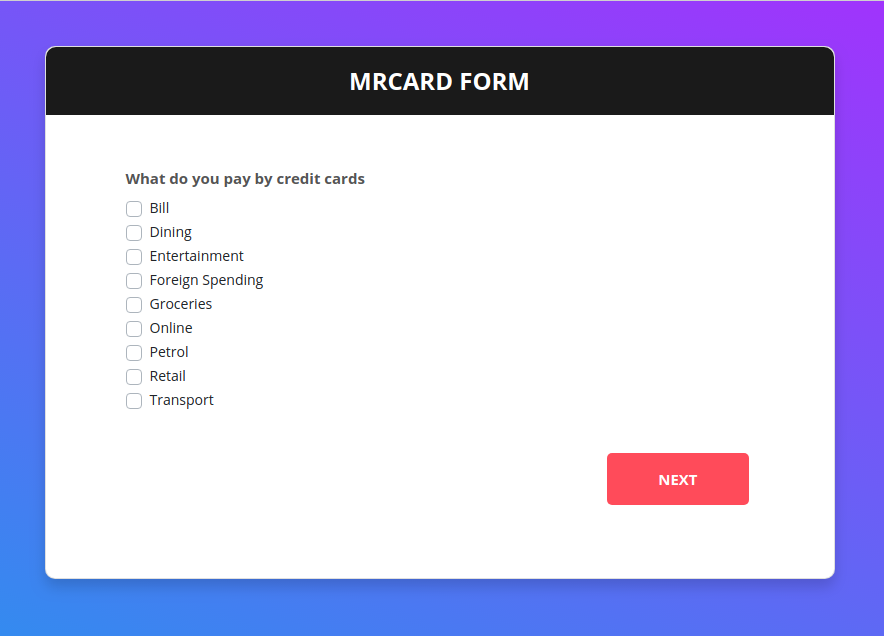
\includegraphics[width=\linewidth]{img/spending_checkbox.png}
		\end{figure}

		Next, please input your spending amounts for each category. You can choose to be as granular as you want or just give a rough estimate (but our calculation will be less accurate then!)

		\begin{figure}[H]
			\centering
			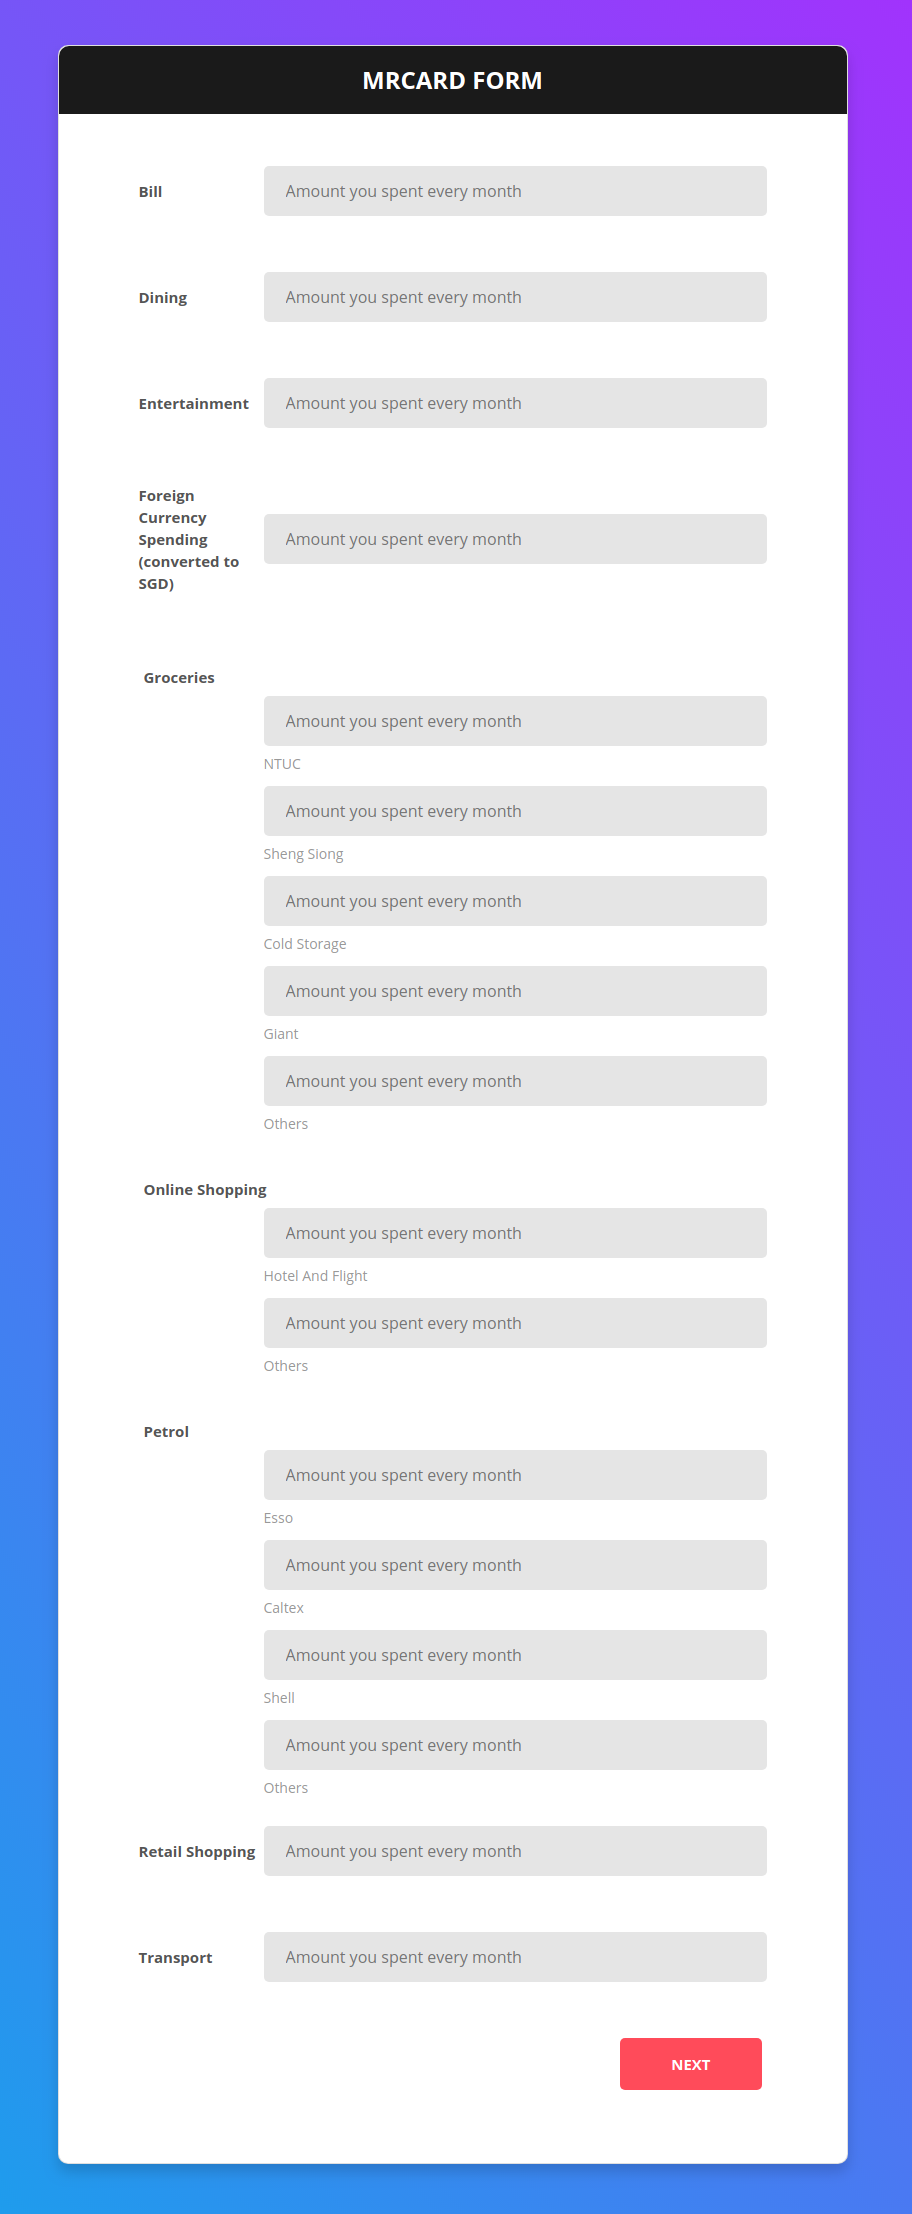
\includegraphics[scale=0.42]{img/spending_amount.png}
		\end{figure}

		And finally based on your eligibility, preferences, spending categories and spending amount, we calculate and give you your recommend ideal and preferred credit card. Click on the Apply button for a link to the official website to sign up! Cheers!

		\begin{figure}[H]
			\centering
			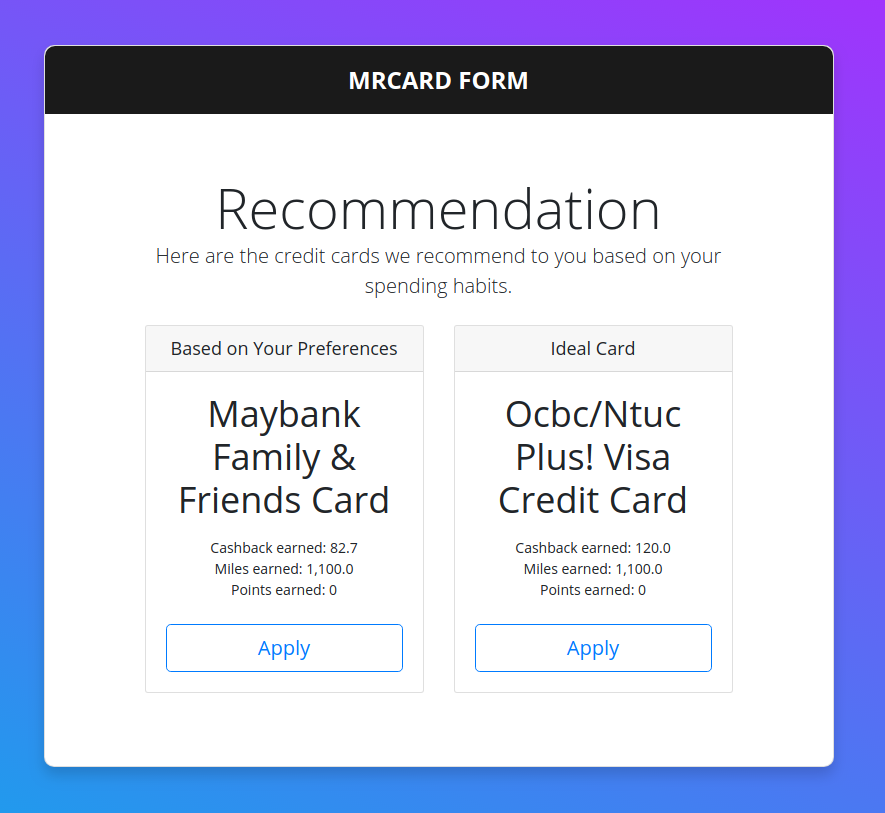
\includegraphics[width=\linewidth]{img/recommendation_v2.png}
		\end{figure}
	% subsubsection start (end)


% subsection appendix_b (end)
\clearpage{}

\subsection{Domain Expert Interview Transcript} % (fold)
\label{appendix:appendix_c}

\begin{description}[leftmargin=4em,style=nextline]
	\item[JH:] Today we would like to thank Hu Jun for attending the interview. We are trying to understand the decision making process on how to choose the credit card or bank card in Singapore.

	\item[HJ:] Hi, my name is Hu Jun. I'm currently a quant researcher in DBS and since I graduated from NUS, I have been using different credit cards and try to explore whether new cards and cards which best my needs. I have been using credit cards for more than 4 years, and so here I am trying to share my experience in choosing credit cards.

	\item[JH:] Okay, thank you Hu Jun. For all the credit cards, do you know who are the target audience for the different credit cards? Do you have a rough category for these cards?

	\item[HJ:] So, it's hard to say there is a clear cut between credit cards because you can classify into different classes or categories by different characteristics. So let’s say, the banks who design credit cards also consider these different perspectives, like what’s the income level of the user, what’s the background of the user, what’s the behavior in terms of the using the credit cards. So, I can say one classification is whether its cash rebate or points based. For cash rebates it's very easy to understand, so you just meet the requirements and you get the cash rebate off your credit card bills. And the other one is you accumulate points, either miles or rewards, then you can choose what kind of reward you want to get, or redeem your points. Maybe it's better for you to ask specific questions so we can zoom in to specific areas.

	\item[JH:] Sure, definitely. So I have a question about the eligibility for different credit cards first. I saw online the the main difference annual income for local is 30k and for foreigner is 45k. But how do you know more about other credit cards, what can it be for the credit card salary limit.

	\item[HJ:] Okay, to me the minimum income requirement is not so strict, because I have tried to apply for different cards and some cards have a high standard of income. At that time I didn’t have that much income but I still got the card. So I think the review process for your application, the focus is on your ability to repay your bills. So as long as you have a good job here in Singapore and you have a stable income every month, even if your income is lesser than the requirement, they will still approve your application, but they may cut your maximum credit limit.

	\item[JH:] Okay. How do you know the maximum credit limit? How do you set the credit limit?

	\item[HJ:] Different banks have different policies. For example, Standard Chartered only give you large credit limit compared to your monthly income. And other bank may have different percentage, some banks may give you 80%, some banks allow you to spend up to 2 or 3 months, if I recall it's around 1 or 2 months.

	\item[JH:] 1 or 2 months, like 1 or 2 months of your monthly salary?

	\item[HJ:] Yes.

	\item[JH:] Is it possible to get some of such information from online?

	\item[HJ:] No. They won't disclose any details of the credit review process. But you should keep updating your particulars because I think most of your target audience are fresh grads who just started to work, but you have just worked for a few months, so they will just give you the minimum amount that they want to give you. And after half a year or one year, you can update your particulars like your last year's CPF or your tax, they will try to upgrade your limit.

	\item[JH:] So actually, our target may be more than the graduate students, may cover all the employee from 25 and above and similar kind of people.

	\item[HJ:] Then your credit record matters. Let's say you never default, you never pay later than the due date, then your points would be very high, they may increase your credit limit.

	\item[LD:] Any advice on how to manage multiple credit cards efficiently? Let's say 4 or 5?

	Okay, first of all I think you need to do an simple analysis of your own monthly spending behaviour ?, then you will know what kind of card fits you best, then you just apply for whatever you need, rather than apply for a lot, then you need to cancel, you need to spend a lot of time to track all your records, because different cards have different requirement, minimum spending requirements, sometimes the bill date is different, you need to check whether you got pay, or it's time for you to spend more on this card to get the waiver for annual fee, these kind of stuff. At the very beginning I tried to apply for different cards, maybe more than 10 cards. Then later I feel that it's a heavy burden for me, then I just try to calm down and just keep maybe 1 credit card for each bank. So, it's around 6 or 7 cards should be more than enough for you to use.

	\item[LD:] Okay. For the annual fee, can we waive every card, or depends?

	\item[HJ:] Normally the strategy is that if they don't provide the waiver for the credit card then you can ask to cancel. But if you want to keep the card, you should keep using it, at least several times, maybe 3-5 times per month and maybe a few thousand each year, then they will keep the card for you.

	\item[LD:] Oh, so they will look at your spending.

	\item[HJ:] Of course, of course. If you never use for the past year, how can you let the customer service officer give you the waiver, right?

	\item[JH:] And for choosing different credit cards, what kind of cards do you need to check by type, by category?

	\item[HJ:] Come again?

	\item[JH:] Like when you choose a credit card, some cards will have cash rebate for certain category, maybe overseas traveling, maybe online shopping. So when we check such information we need to put into such categories for the user to input. What should they be, when we want to ask them to put these information?

	\item[HJ:] Ask who to put?

	\item[JH:] The user, to put these information in our system to get the recommendation.

	\item[HJ:] Okay. First of all you need to get the terms and conditions for each card, it's quite troublesome because different banks classify different spending type into different groups. So let's say cashback, normally they will put dining, maybe online spending, and supermarket, these are maybe common classifications, but some banks just have differences. It varies from bank to bank, so when you try to calculate the categories, the caps and how to meet the minimum requirement, it's quite troublesome, you need to fit all the terms and conditions, and banks sometimes change them like half a year or 3, 4 months. So for me at the very beginning I used to keep track of my own spending to meet all the requirements, later feel it’s quite troublesome. I don’t want to spend too much time on it so I came back to the miles card.

	\item[JH:] Miles card are easier to manage.

	\item[HJ:] Yes. So for people who don’t want to spend too much time on it, just use this kind of miles card like Citi Miles, DBS Altitude , maybe American Express, KrisFlyer credit card.

	\item[JH:] For miles they have like certain multiplier to calculate how much miles to give for each Singapore dollar right? For the rewards it looks like they have similar calculation. How could they be different between the miles and the rewards card?

	\item[HJ:] So normally I think it’s more or less the same, so for me, if you want to compare between different credit cards, you need to develop a system which can convert your rewards to percentage. Let’s say a miles card right, normally in Singapore you spends locally 1 dollar, you can get back 1.2 miles, then you should try to convert into percentage, you try to estimate how much miles you need to get a redemption ticket. Then you try to estimate the value of the ticket, then you try to convert back, you treat the ticket value as the rebate, then you try to calculate if you want to get this ticket, how much money you need to spend by using this card. Then you get the percentage, then you can compare between the different cards.

	\item[JH:] So you mean to change the miles into cash value so we can keep comparing.

	\item[HJ:] Yeah, but it depends on how do you want to use your miles or rewards points. Let’s say every time you redeem your business class air ticket, definitely the rebate rate is much higher than the economy one, because the ticket value is higher, it’s not a linear relationship.

	\item[JH:] What do you mean by this?

	\item[HJ:] Let’s say we get a Singapore airlines ticket from Singapore to Beijing, then you need maybe 20k miles for economy class right? But the ticket will be around \$400. But if you use 40K miles to get a business class, the ticket value may not be \$800, it might be \$1000 dollars. So it’s different. So first of all you need to know if you get these rewards, how you want to use it. Normally your behaviour is to redeem a business class tickets or an economy class, then if you saw the real value of the points for you and for another person who redeem different air ticket class, it’s very different.

	\item[JH:] Do they have like certain trend like, if I redeem less and get a cheaper ticket, the rate may be low, if I redeem more and get business or first class …

	\item[HJ:] First class returns is definitely better.

	\item[JH:] So it means if you use more air miles you get a higher rebate value.

	\item[HJ:] Yes.

	\item[JH:] And for the air miles, can they only redeem the tickets, or can they also redeem others?

	\item[HJ:] Others also can. You can off your bills, you can choose different gifts from maybe either Singapore airlines or alternatives. You can go to the shops. Let’s say you have the DBS card, there is a reward program that’s there, then you can choose whatever you want by using your points to redeem and you could get the gift.

	\item[JH:] So it means if you have such miles, it works exactly as the miles in that airline’s website.

	\item[HJ:] Not really, if you are using let’s say DBS card right, the redeem website is developed by DBS, so you can choose using this website. But if you convert or transfer your reward points, miles to Singapore airlines, your choice will be decided by Singapore Airlines.

	\item[JH:] So it depends on how they connect the system with the miles?

	\item[HJ:] No, it depends on where you want to spend it before the transfer or after transfer. After transfer is chargeable.The choices will be provided by Singapore airlines. But if before the transfer, the choices are provided by the bank who issued this credit card.

	\item[JH:] Normally which is better?

	\item[HJ:] I didn’t compare, but last time I think I tried to calculate the return value, air ticket is more efficient in terms of value , because I used to redeem air ticket during departure, come back around a hot season, so at that time if you use cash to buy, let’s say from Singapore to Beijing, it’s normally \$400, sometimes during Chinese new year it’s about \$600 or \$800, so they rebate will increase.

	\item[JH:] And for the redemption, will it change for the season, like if it’s the hot season?

	\item[HJ:] No. sometimes it has promotions and give you discount. But normally if they set 20k for example . Before the next change it will stay as 20k, regardless of the time you want to travel.

	\item[JH:] So you just mentioned there will be a conversion fee to the bank miles and the real airline miles rights?

	\item[HJ:] Yes, only if the card is issued together by the bank and the airlines. For example, American Express Singapore Airlines card. That one will automatically transfer the miles for you every month without charging you anything. For the rest you need to pay, and it must be like for every 5k transferred or every 10k transferred, you cannot transfer and amount you want.

	\item[JH:] And for every transfer you need to pay the…

	\item[HJ:] Around twenty to thirty dollars. Processing fee.

	\item[JH:] Who will decide whether it be, by the airline or?

	\item[HJ:] By the bank.

	\item[LD:] For the airline, the redemption of the air ticket, are there a lot of terms and conditions? Or are you free to redeem anywhere and anytime you want?

	\item[HJ:] There are some restrictions, but it’s not terms and conditions. So in terms of terms and conditions, most of the tickets you cannot change, I think, but I cannot remember, you can check the website. Normally, every flight they have a quota, quota meaning only 10 tickets can be redemption tickets, then if it already has been redeemed by other people, you need to wait on the waiting list.

	\item[JH:] How do they define this quota? By month or by year?

	\item[HJ:] I am not sure. Last time round I called customer service of Singapore Airlines, they refused to answer this question. But there definitely is a quota. Cannot be everybody on the flight is redemption ticket.

	\item[JH:] For these air miles will they expire after certain years.

	\item[HJ:] If in your bank account, most of the banks will keep it as long as you want. But if you transfer to airlines, normally they will have 2 or 3 years expiry.

	\item[JH:] For some card you mentioned they (Banks and Airlines) cooperate together  for such card, and then they will automatically transfer right, and the expiry depends on the airline.

	\item[HJ:] Yes, same. As long as in the airlines account it will expire.

	\item[JH:] For airline, getting the miles through your spending directly, and then recommend the category sometimes, different mile calculation right? And do they have a * yet for most credit cards?

	\item[HJ:] No.

	\item[JH:] So you can spend as much as you want, and get as much miles as you want?

	\item[HJ:] Yes.

	\item[JH:] For the rewards, the rewards card looks the same as the miles, what can they use the points for?

	\item[HJ:] It differs from card to card, I need to check the details, but you can use the same methodology to try to calculate the return, then you choose which kind of reward you want to get.

	\item[JH:] What’s the normal reward for the rewards card? And also miles cards, the airline ticket?

	\item[HJ:] I think if you want to apply for a credit card, the minimum should be 1\%, and it can be maybe up to 4\%, 5\%, that the maximum. And for those kind with high rebate rate cards, they always put a lot of restrictions, like minimum spent, and maybe you need to link to your savings account, and maybe you need to credit your monthly salary into that account, all those kind of stuff. Because there are enough competitor in the market, so the rates should be more or less the same.

	\item[JH:] So it mean that the cash rebate is better than the airline or rewards, if you can get that rebate.

	\item[HJ:] Not really, it depends on how you spend the reward points. So let’s say you use your credit card which is either reward or miles, every time you redeem first class air ticket, definitely your requirement will be a bit better than your cash rebate. Cash rebate is fixed one, you don’t have a choice.

	\item[JH:] Can you give me some example of how you can use these rewards?

	\item[HJ:] You can buy almost anything you want. So it’s like if you want to use your reward point to buy electronics, you want to buy air ticket, you want to buy souvenirs or you want to buy some luxury items, there are a lot of choices for you actually. And you can get some vouchers like NTUC or Takashimaya, Robinsons, even some like haircut, like QB House also can. So a lot.

	\item[JH:] So you need to use the rewards to get the vouchers first.

	\item[HJ:] Yes.

	\item[JH:] And all the voucher redemption is based on the bank.

	\item[HJ:] Yes.

	\item[JH:] Ok

	\item[JH:] For the cashback, do you have any recommendations at the moment? Normally, what kind of limit will they set? Is it quite different for different cards?

	\item[HJ:] I have abandoned all the cashback cards because, only one I’m using is UOB, because it’s quite simple, it seldom changes the calculation for your rebates. And they don’t have category. I mean they don’t need you to spend in different categories in order to get the rebates, and the rebate category got a cap. So normally like the Citi Cashback card, they have several categories. First you need to fulfil the minimum spent on this card, then in order to maximise on the return, you need to spend the exact number in each category to get the rebate. Also as you overspend that category, the cash rebate rate will be very low. So it’s quite troublesome you need to keep track of this card, you need to keep track of spending category in this card, spend much time to get the rebate. So it’s easier to use cards like UOB ONE, where you just need to meet the minimum spent, then that’s all you get the rebate, you just need to remember how much you spent on this card, that’s all.

	\item[JH:] It seems that cash rebate card has some…

	\item[HJ:] And another flaw for this card is they always change the category. Sometimes they just adjust for this category, and may increase the rebate rate, for other category, it may reduce the cap, all those kind of stuff, and if you don’t have the latest information, your spending will be wrong, you don’t get the maximum of the rebate.

	\item[JH:] I know that there are many cash rebate cards that may cooperate with some different malls or some different canteen to get higher rebate right?

	\item[HJ:] Yes but it’s changing all the time. So maybe every 3 months they will change, maybe 1 year. It depends, it really depends. So that’s another reason for you to keep multiple cards, every time you don’t consider which restaurant to eat at, if you dine there, you got some rebate, you just go there and you check whether you have that card or not. If you have that card you just get the promotion rate.

	\item[JH:] So for lazy people, what the best choice for them? Air miles cards?

	\item[HJ:] Air miles cards.

	\item[JH:] If I am the lazy people and I do not want to calculate the cash rebate or this or that so the best choice is air miles card right? Or maybe rewards?

	\item[HJ:] Hmm, rewards. You can choose miles card because, for example if you want to pay your tuition fee, or maybe insurance, this card may give you certain miles. But for most cards, if you pay for these kind of stuff, they never issue miles to you. I think you should at least have two. One is cash rebates and one is miles. So let’s say the cash rebate card, the minimum spending requirement is \$1 right. You just spend \$1000 on this card, and then the rest you just use the miles card, you don’t have to do any calculation.

	\item[JH:] Okay, got it. So the best choice may be a combination with cash rebate and miles.

	\item[HJ:] Yeah. But it always comes back to the very first recommendation I mentioned, you need first to analyse your spending. If you spend a lot on online shopping then definitely you should have cash rebate or whatever card that focuses on online shopping.

	\item[JH:] So we need to know how the user spend their card\/money the week or month before.

	\item[HJ:] Yes, of course.

	\item[JH:] So this also requires you to know how to manage multiple credit cards efficiently right?

	\item[HJ:] Yes.

	\item[JH:] Also, since this is all about credit cards, we want to know how these banks work. What are the different types of bank account in Singapore can be? Like for savings, for current account . Do you have a understanding on that?

	\item[HJ:] So I think most of use just need a savings account because it give you interest. For current account there is no interest. Only if you need to have a lot of transactions, like withdrawals and deposits, then you use a current account. There’s no limit or maximum number you can transact with this account. So for normal people you just have a savings account, that’s enough.

	\item[JH:] So the current account is not used by people quite often.

	\item[HJ:] Most of the time its companies. It’s a working account, like you transact a lot, like a thousand time a month.

	\item[JH:] For the savings account, I know that for different bank they also have a special program to get the high interest. Can you share some information on that, how it works for most banks?

	\item[HJ:] Okay more or less it’s the same, because some banks they may just have a new account, maybe have a promotion, and later if they have attracted enough people, I mean enough amount of money, they will change the policy. And they try to lock you, because you have already link salary to this account, so they just reduce the rebate or whatever. So, currently I prefer UOB because UOB is stable, they don’t want to change. And as far as I know, I think OCBC and BOC also got this kind of saving account but you need to credit your salary, you need to have maybe investment or insurance with this bank.

	\item[JH:] For the investment in the bank, how does it work? Will they give you a positive return every year?

	\item[HJ:] Depends on what kind of investment you are using. If you choose bonds, most of the time it’s positive, but if you choose equities, how do we know?

	\item[JH:] So what the general rule for bank doing this? What’s the minimum requirement for one savings account? Do they have a rough number?

	\item[HJ:] Savings account? No.

	\item[JH:] You mentioned for investment they will give you a certain interest rate right?

	\item[HJ:] Your requirements are for what?

	\item[JH:] Requirements to fulfil the high interest rate for the saving account by fulfilling some of the events.

	\item[HJ:] Oh okay. The only one I know for the moment is OCBC. OCBC if you have investment in the bank, they will give you extra bonus interest rate like 1.8? I don’t know.

	\item[JH:] And also for the insurance are similar?

	\item[HJ:] Similar as well. They just want to sell you more products, and make more money from you.

	\item[JH:] Insurance is also mainly from OCBC or other companies as well?

	\item[HJ:] Insurance only for OCBC at the moment. Normally banks want you to credit your salary into the account, want you to set up GIRO, maybe want you to increase the amount you save there every month. Oh and you need to have a credit card spend the minimum requirement.

	\item[JH:] Actually for banks they have savings account and different debit card and credit card. Do they have a connection? Except this bonus part. Do you need to get a savings account for debit card?

	\item[HJ:] For debit card yes, for credit card no. Credit card is an independent account, but debit card you need to have money in the bank then you can debit right. So you must set up a saving account in the bank, then you link your debit card to the account. But nowadays you can link your credit card to the account.

	\item[JH:] So it’s not necessary to have debit card nowadays.

	\item[HJ:] Yes, there is another kind of card which is called the ATM card.

	\item[JH:] So for the ATM card, do all the banks provide, or depends on what are the type of bank you are using

	\item[HJ:] I think most of the banks provide it, because at the very beginning you may just want to deposit and withdraw money from the bank, you just need ATM card, you don’t need ant NET, Visa, Master, or whatever. Then you don’t need a debit card. I think the only difference between a debit card and an ATM card is it provide this kind of payment channels.

	\item[JH:] So now I have a credit card, and if possible I want to put the ATM card in my credit card.

	\item[HJ:] It’s not put into, you just link your credit card to your savings account, and withdraw money.

	\item[JH:] And there are no additional fee for that?

	\item[HJ:] No.

	\item[JH:] So it means I can cancel all my debit cards?

	\item[HJ:] Yes. But some debit card like DBS, Platinum debit card, you can have 5\% rebate when you use PayWave. So these kind of debit card we want to have it.

	\item[JH:] But for the DBS, they only provide such rebate for debit card not for credit card.

	\item[HJ:] No. Interesting.

	\item[JH:] We are building a system for recommending different credit cards, and even the saving account if we have time. We have a challenge, which is how to choose multiple credit cards by getting the person’s spending habit. The thing is, we do not know how to divide the amount to match different calculations inside. And recommendations?

	\item[HJ:] Generally it’s an optimisation problem. You need to design the function you want to optimise. For your problem I think it’s quite easy. Total amount of rebate, or maybe total return or the rate of your rebate. So, your input should be the different amount to different credit card.  Try to optimise the inputs, to maximise the outputs, the return rate should be okay. But I think the challenging part is how do you do the conversion, the points into the return rate. And you need to decide which product or gift you want to redeem by using the points.

	\item[JH:] Do you think there is a simple way, like we just fulfill the first card, and then deduct the amount to try to optimise to get the other card.

	\item[HJ:] No, I think it’s going to be a more risk kind of thing. You need to do analysis and understand the terms and conditions for each card.

	\item[JH:] So to simplify this problem, you mentioned it’s better to use all you spending in one rebate card first, and one it reach certain amount or cap, then you use other amount in miles. It’s easier to relook such problem.

	\item[JH:] Okay, thank you.

	\item[LD:] Thank you.

	\item[HJ:] Thank you. All the best for your project.

\end{description}

\clearpage{}
% subsection appendix_c (end)

\subsection{Project Related Files} % (fold)
\label{sub:project_related_files}
	\textbf{Presentation Video:} \url{https://youtu.be/vu1eQ-0R4e8}

	\textbf{Interview Audio:} \url{https://github.com/davidygp/IRS-MR-2019-01-19-IS1PT-GRP-MRCard/blob/master/Miscellaneous/Interview%20with%20Hu%20Jun.mp3}

	\textbf{Attribute Table:} \url{https://github.com/davidygp/IRS-MR-2019-01-19-IS1PT-GRP-MRCard/blob/master/Miscellaneous/Data%20Fields%20-%20Sheet1.csv}

	\textbf{Bank Data:} \url{https://github.com/davidygp/IRS-MR-2019-01-19-IS1PT-GRP-MRCard/blob/master/Miscellaneous/Card%20Data%20-%20Bank%20Card%20Data%20(Cleaned_v2).csv}

	\textbf{Survey Result:} \url{https://github.com/davidygp/IRS-MR-2019-01-19-IS1PT-GRP-MRCard/blob/master/Miscellaneous/MRCard%20Survey%20Result.xlsx}


% subsection project_related_files (end)


% section appendices (end)